\documentclass[11pt,a4paper]{article}
%\documentclass[article] {report}
%\documentclass[titlepage]{report}
\usepackage[utf8]{inputenc}
\usepackage[catalan]{babel}
\usepackage{amsmath}
\usepackage{amsfonts}
\usepackage{amssymb}
\usepackage{verbatim}
\usepackage{float}
\restylefloat{table}
\usepackage{adjustbox}
\usepackage{lscape}
\usepackage{graphicx}
\usepackage{tikz}
\usepackage{pgfplots}
%\usetikzlibrary{plotmarks}
\usepackage{subcaption}
\usepackage{enumerate}
\usepackage{afterpage}
%\usepackage{gantt}
%\usepackage{pdflscape}
\usepackage{pgfgantt}
\usepackage[left=4cm,right=4cm,top=4cm,bottom=4cm]{geometry}
%\pgfplotsset{yticklabel style={text width=3em,align=right}}
\pgfplotsset{
	%ylabel style={overlay},
	%yticklabel style={overlay},
}
\usepackage{lipsum}

%\title{Millora de rendiment d'un sistema d'avaluació de traductors automàtics}
%\date{22 d'abril de 2015}

\begin{document}

%\maketitle
\begin{titlepage}
    \begin{center}
        \vspace*{4cm}
        
        \LARGE
        Millora de rendiment d'un sistema d'avaluació de traductors automàtics
        
        \vspace{0.5cm}
        \large
        22 d'abril de 2015
        \vfill
        
    \end{center}
\end{titlepage}

\afterpage{\null\newpage}


\newpage
\begin{abstract}
Memòria del TFG \textit{(Treball Fi de Grau)} ``Millora de rendiment d'un sistema d'avaluació de traductors automàtics''.
\\

Autor: \textit{Ibai Gilabert Rodríguez}

Direcció: \textit{Jordi Turmo Borras}

Codirecció: \textit{Meritxell González Bermúdez}

\end{abstract}


\newpage
\tableofcontents
\newpage

\section{Introducció}

Aquest projecte s'emmarca dins l'àrea del processament del llenguatge natural \emph{(NLP)}, que és alhora una àrea d'estudi en el camp de la Intel·ligència Artificial. Aquest àrea abasta un ampli ventall d'aplicacions pràctiques, entre elles la traducció automàtica.
\\

Podem definir que una \emph{bona} traducció és aquella que expressa el mateix significat que el text original. Degut a la riquesa del llenguatge moltes oracions poden expressar el mateix amb paraules molt diferents. Alhora de discernir el significat d'un text entra en joc la valoració personal i totalment subjectiva de cadascú per analitzar conceptes tant difosos com el context, la coherència del text o l'eloqüència... 
\\

La ``traducció'' és una tasca especialment complexa ja que mesurar la \emph{qualitat} d'una traducció és un concepte molt vague. De fet, fins i tot entre els humans no hi ha consens alhora de definir o estipular \emph{com} es mesura o sota quins barems s'ha de jutjar una traducció. A més, la manera de \emph{mesurar} pot variar significativament depenent de factors molt diversos (la finalitat del text, el gènere, etc).
\\

%Per aquest motiu, l'avaluació manual d'una traducció és lenta i costosa, i per tant, difícilment sistematitzable
Sembla evident que no podem quantificar res de tot això de manera sistemàtica; podem fer-ho manualment però l'avaluació manual d'una traducció és una tasca lenta i costosa i, per tant, difícilment automatitzable. Per això s'investiga en \textit{com} quantificar la qualitat d'una traducció de manera automàtica. Actualment es possible fer estimacions mitjançant mètriques d'avaluació automàtica.
\\

En l'actualitat existeixen moltes d'aquestes mètriques d'avaluació, i totes elles de complexitat ben dispar. Algunes, per exemple, són simples comptadors de n-grames i altres poden incloure sintàctics i semàntics o fins i tot mètodes molt sofisticats d'aprenentatge automàtic.
\\

Degut a la naturalesa del problema, es pot preveure que aquesta és una tasca de gran complexitat computacional.
\\

L'objectiu d'aquest projecte és millorar el rendiment d'\texttt{ASIYA}, una plataforma d'avaluació de traduccions automàtiques que es descriu en detall a continuació.

\subsection{Context}
%Prenem com a \textit{baseline} un sistema plenament funcional: ASIYA\cite{asiya}.
%\\

\texttt{ASIYA}\cite{asiya} és una plataforma de codi obert per a l'avaluació de la Traducció Automàtica \emph{(MT evaluation)} i meta-avaluació. Disposa d'un conjunt considerable de mètriques per a la mesura de la qualitat de la traducció automàtica en diverses dimensions lingüístiques, incloent l'anàlisi sintàctic i semàntic.
\\

\texttt{ASIYA} és una eina que posa a disposició un ventall molt ampli i heterogeni de mètriques d'avaluació i meta-avaluació (avaluació de mesures d'avaluació automàtica), la majoria d'elles són usables i perfectament vàlides per a ser executades de manera singular. Així que \texttt{ASIYA} actua més aviat com una plataforma per facilitar l'ús de tota aquesta disparitat de mètriques. El principal problema és la ineficiència. Aquesta ineficiència procedeix del comput seqüencial de càlculs molt lents i amb requeriments de memòria dispars.
\\

A continuació definim breument les dades amb les que treballa {ASIYA}.
\\

%\paragraph{Input} Conjunt de documents agrupats en 3 categories diferents: conjunt de documents en llengua origen \textit{(source)}, traduccions humanes associades a cada \textit{source} en llengua destí \textit{(reference)} i traduccions automàtiques en llengua destí de cada document per a cada traductor automàtic dins d'un conjunt de traductors automàtics \textit{(system)}. Aquests inputs poden venir donats en diferents formats. ASIYA els adaptarà per tractar-los en format text.

\paragraph{Input} Un text en la llengua origen \textit{(source)}; un conjunt de traduccions humanes en la llengua destí \textit{(reference)}; i un conjunt de traduccions automàtiques produïdes per diferents sistemes \textit{(system)}. Cada text consta d'un o més documents, i cada document està format per una o més oracions (segments). Aquests inputs poden venir donats en diferents formats. \texttt{ASIYA} els pre-procesa per tractar-los en format text.

%\paragraph{Output} ASIYA generarà una puntuació \textit{(score)} per a cada sistema i cada mètrica amb 3 nivells de granularitat: segment (oració), document i sistema. Aquests \textit{scores} es desaran en fitxers comprimits amb la finalitat de no repetir càlculs en execucions posteriors.

\paragraph{Output} \texttt{ASIYA} és capaç de calcular diferents mesures de qualitat \textit{(scores)} per a cada traducció automàtica. Aquests \textit{scores} els proporcionen les mètriques integrades dins d'\texttt{ASIYA} que, a la vegada, poden obtenir mesures de qualitat a nivell de segment, document o sistema (tot el text d'entrada).

\paragraph{Paràmetres} S'ha de proporcionar un fitxer de configuració amb les mètriques que voldrem executar. Aquestes mètriques es poden agrupar en ``families'' o \textit{metric sets} per a millor confort.
\\

L'actual versió d'\texttt{ASIYA} no contempla cap mena de seqüenciació en paral·lel. Tota l'execució es realitza successivament per cada mètrica i per cada sistema.
\\

En l'actualitat no hi ha cap eina o plataforma, per quantitat i qualitat, com \texttt{ASIYA}, com a mínim d'aquestes característiques. No obstant, el seu principal handicap són els recursos que exigeix. Tot i que algunes mètriques fan ús d'eines externes com ara processadors lingüístics que, per motius de manteniment i flexibilitat no toquem i tractem com a caixes tancades i completament opaques, sí és cert que es deixa entreveure una certa concurrència en el càlcul dels \textit{scores}, derivat de fragmentar els inputs. Així com també és concurrent l'execució de moltes mètriques ja que la majoria són completament independents entre elles.
\\

És a dir, concurrència a nivell de mètrica i concurrència a nivell de document.
\\

Aquest és el principal objectiu del projecte. Com podem fragmentar l'execució d'\texttt{ASIYA} de manera que mitjançant alguna arquitectura paral·lela millorem l'ús dels recursos?

\subsection{Abast}

Com ja s'ha esmentat \texttt{ASIYA} és una eina flexible, adaptable i de fàcil integració. Això és una característica que no volem perdre.  Això vol dir que les tasques de manipulació de l'eina com afegir mètriques, llengües; modificar formats, etc han de ser el més fàcils possible. Es persegueix una filosofia o idea de senzillesa en el seu ús i edició. Adaptabilitat al cap i a la fi.
\\

Donada una entrada definida per l'usuari, \texttt{ASIYA} calcula cada puntuació \textit{(score)} de manera consecutiva i processa cada traducció oració per oració, per a cada document de cada sistema i conjunt de mètriques. La majoria de \emph{scores} són a nivell d'oració i completament independent entre ells. Per tant, aquests poden ser calculats de manera paral·lela.
\\

Així doncs, per a modificar la metodologia de còmput, el que ens queda es modificar el tractament de les dades. Com a primera presa de contacte podem definir el nostre posicionament de la següent manera: si tenim una entrada de mida $N$ (oracions) la partirem en $n \leqslant N$ fragments perquè \texttt{ASIYA} pugui executar aquests fragments de manera paral·lela. Aquesta és la idea.
\\

Per portar-ho a terme, es plantejarà un re-disseny íntegre de tot el sistema ja que la versió actual no està preparada per a cap mena de paral·lelisme. Amb aquesta intenció escollirem un llenguatge més adient per a les nostres necessitats (eficiència i concurrència). S'ha escollit \texttt{C++} per la seva estructura de classes, tipificació i compatibilitat amb diferents paradigmes de programació paral·lela que veurem en la següent secció.
\\

% % % % % % % % % % % % % % % % % % % % % % % % % % % % % % % % % % % % %
% % % % % % % % % % % % % % % % % % % % % % % % % % % % % % % % % % % % %
% % % % % % % % % % % % % % % % % % % % % % % % % % % % % % % % % % % % %
% % % % % % % % % % % % % % % % % % % % % % % % % % % % % % % % % % % % %
% % % % % % % % % % % % % % % % % % % % % % % % % % % % % % % % % % % % %
\newpage
\section{Estat de l'Art}
El projecte està orientat a la millora de rendiment d'un sistema d'avaluació de traduccions automàtiques, \texttt{ASIYA}. Tot i que sigui d'una aplicació concreta, aquesta només és el punt d'inici per a la consecució dels objectius marcats. Per tant, amb la intenció de mantenir aquests objectius clars i realitzables hem decidit que l'estat de l'art dels mètodes d'avaluació queden fora de l'abast del projecte donat que no estem desenvolupant un mètodes d'avaluació sinó millorant el rendiment d'una eina.

\subsection{Models de computació paral·lela}
Com es cita a la secció anterior, la proposta és paral·lelitzar el tractament de les dades. Donat l'entorn en què es desenvoluparà l'eina, tenim dos possibles models de paral·lelització: \textit{GPU} (secció 2.1.1) o Clúster de computació (2.1.2)

\subsubsection{\textit{GPU Computing}}
En un inici, el paradigma de computació paral·lela en GPU va ser ideat per a resoldre una necessitat imperiosa de càlcul cada vegada més massiu amb l'objectiu de produir gràfics més realistes. Aquesta motivació es veu reflectida en l'arquitectura. Totes les GPUs comparteixen un filosofia de disseny orientada a solucionar càlculs molt repetitius de manera massiva propis del món gràfic.
\\

\begin{figure} [!h]
\centering
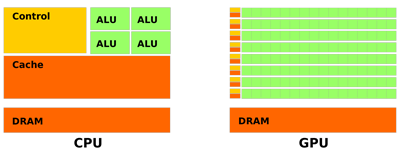
\includegraphics[width=10cm]{resources/cpu-gpu_w.png}
\caption{CPU-GPU, conceptes diferents}
\end{figure}

Entrant una mica més a fons en l'arquitectura GPU, el detall que, d'entrada pot provocar certa perplexitat, és el nombre de nuclis que conté. És una qualitat característica que a priori pot semblar  miraculosa\footnote{Una GPU de gamma mitja actual sobrepassa els 1000 \textit{cores}.}. Cal destacar que no són \textit{cores} en el sentit clàssic del vocable informàtic (unitats de propòsit general, amb unitat de control, entrada/sortida, etc). Aquests nuclis s'assemblen més aviat a ALUs \textit{(Arithmetic Logic Unit)}. És a dir, a petits coprocessadors destinats exclusivament al càlcul numèric.
\\

La història de com aquestes unitats van transcendir l'àmbit gràfic per constituir-se com a alternativa real per a programes de propòsit general  és molt interessant. Els exemples més recurrents són aplicacions científiques en l'àmbit de la recerca (bioinformàtica, química computacional..), i també empresarial (simulació de fluids, etc)\cite{CUDAapplications}. De fet, els principals fabricants, especialment NVIDIA, ja fa anys que presenten solucions d'altes prestacions no orientades al \textit{rendering}.  Es poden aconseguir resultats de super-computador de petita escala en un ordinador personal.
\\

\begin{figure} [!h]
\centering
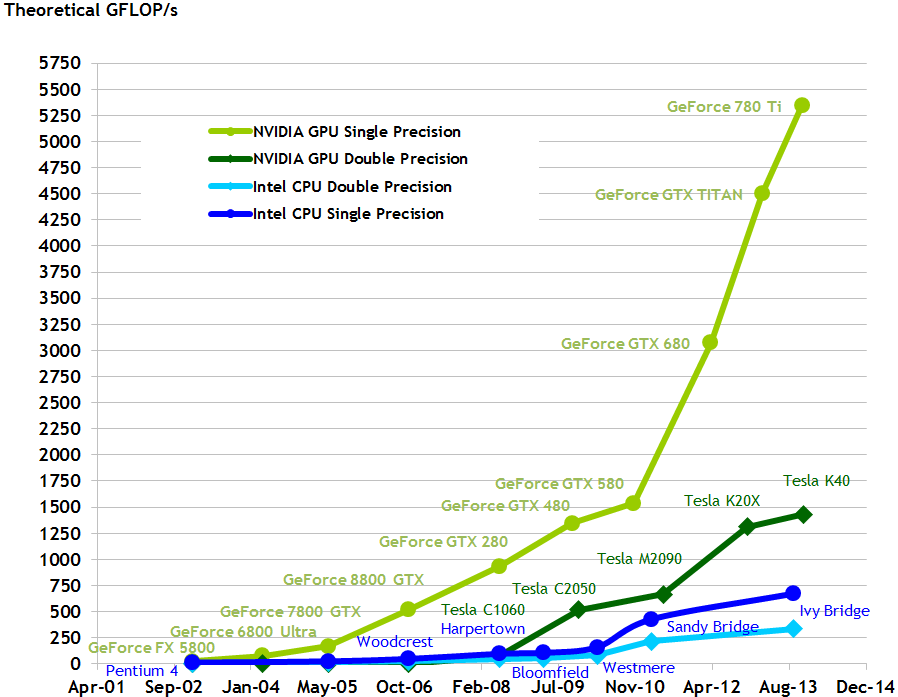
\includegraphics[width=12cm]{resources/floating-point-operations-per-second.png}
\caption{Comparativa de rendiment en \textit{FLOPS}}
\end{figure}

NVIDIA presenta una gamma de GPUs dedicada al segment de la supercomputació anomenada ``Tesla''\cite{tesla}. El RDlab disposa actualment d'aquestes GPUs.
\\

Pel que fa a la programació amb GPUs, existeixen vàries plataformes: algunes lliure com OpenCL\cite{opencl}; i altres tot i ser gratuïtes, com en el cas de NVIDIA, només són aptes en les seves targetes. L'API que ofereix NVIDIA per a la programació amb les seves targetes s'anomena CUDA\cite{cuda}.
\\

Podem afirmar amb rotunditat que el model GPU representa el màxim exponent de la computació paral·lela, ja que des de els seus inicis va ser pensada per aquesta finalitat.
\\

Tot i disposar d'aquest recurs l'hem descartat per a l'alta ``especificació'' que exigeix adaptar el codi a l'execució amb GPUs. És a dir, modificar el codi \emph{ad hoc} per a CUDA el fa poc reusable i per al projecte només és apte per a càlculs molt concrets en determinades circumstàncies. Degut a la dependència que establim amb les mètriques externes, amb les quals hem pres el compromís de no modificar-les i, a més, estan implementades en diferents llenguatges, la opció GPU no és vàlida per al nostre cas.
\\

A més, la via GPU té una limitació intrínseca i és la limitació de la memòria de la targeta. Un problema que no tindrem, o no serà tant crític, en la següent proposta.

\subsubsection{Clúster de computació}
Mastodòntics és un bon adjectiu per a descriure els recursos que molts procediments de tractament del llenguatge natural exigeixen. Ja s'ha comentat la necessitat d'un entorn d'execució d'altes capacitats. Per aquestes tasques de recerca i altres l'any 2010 va néixer el \textit{Laboratori de Recerca i Desenvolupament} (RDlab). Aquest ofereix un entorn ideal per a les nostres necessitats: \textit{``El nostre clúster de computació d'altes prestacions (HPC) proporciona un entorn perfecte per execucions massives''}\cite{cluster}.
\\

Aquest sistema implementa un \textit{Sun Grid Engine}. El clúster el composen una seguit de nodes (independents entre ells i absolutament autònoms). Cadascun d'aquests nodes disposa d'uns recursos hardware variable (i en constant actualització). Per fer ús del sistema els usuaris envien tasques \textit{(jobs)} i aquest les encua i les enviarà a executar seguint una sèrie de paràmetres (disponibilitat, prioritat, etc) als nodes que s'escaiguin.
\\

Aquest mecanisme ens permet executar \textit{jobs} amb els quals crear altres \textit{jobs} que idealment s'executaran de manera paral·lela (el sistema de cues s'encarregarà de la planificació de recursos).
\\

Així doncs, podem plantejar la implementació de la concurrència de la següent manera: 
\begin{enumerate}[1.]
    \item Llançar \texttt{ASIYA} en mode paral·lel. Aquest, fragmentarà les dades d'entrada de manera adient.
    
    \item Aquest mateix procés encuarà més processos \texttt{ASIYA} per a cadascun dels fragments a tractar.
    
    \item Quan els subprocessos hagin acabat, l'\texttt{ASIYA} (pare), que estava esperant, llegirà els fitxers amb els resultats de les execucions dels \texttt{ASIYA} (fills). I, si fos el cas (es demana \emph{score} a nivell de document o sistema) calcular els resultats finals amb tots els resultats parcials (\emph{scores} a nivell d'oració).
\end{enumerate}

Entenent que és de menester un sistema \texttt{HPC} i essent aquesta la millor opció que tenim al nostre abast, aprofitarem aquesta tecnologia amb la intenció d'implementar el paral·lelisme que desitgem. 
\\

Descartada l'opció GPU hem apostat per aprofitar la tipologia del clúster per a una solució que implementi el paral·lelisme de manera ``recursiva''.  La idea fonamental és que si donada una entrada determinada i indicant-li a \texttt{ASIYA} que s'executi de manera paral·lela, llavors processarà l'entrada, la partirà de la manera desitjada i encuarà tants processos \texttt{ASIYA} (seqüencials) com sigui necessari tenint en compte el nombre de mètriques, documents i mida d'aquests. Un cop s'hagi acabat els càlculs parcials, \texttt{ASIYA} els recull i genera la solució final. Podem veure-ho com un \texttt{ASIYA} \emph{master} invocant múltiples \texttt{ASIYA} \emph{slaves} ja que, \textit{de facto}, actuen d'aquesta manera.
\\

En la següent secció veurem la planificació de les principals tasques que composen el projecte. Així com la seva planificació.


% % % % % % % % % % % % % % % % % % % % % % % % % % % % % % % % % % % % %
% % % % % % % % % % % % % % % % % % % % % % % % % % % % % % % % % % % % %
% % % % % % % % % % % % % % % % % % % % % % % % % % % % % % % % % % % % %
% % % % % % % % % % % % % % % % % % % % % % % % % % % % % % % % % % % % %
% % % % % % % % % % % % % % % % % % % % % % % % % % % % % % % % % % % % %
\newpage
\section{Planificació}
El projecte es durà a terme seguint un esquema bàsic de prototipatge. Desenvoluparem 2 prototips.
\\

A continuació detallarem cadascuna de les tasques a realitzar.

\subsection{Requisits d'usuari i disseny}
En aquesta fase es pretén analitzar els requeriments i l'especificació de la nova versió \texttt{ASIYA}. L'objectiu és estudiar les diferents alternatives hardware i de disseny per escollir la millor opció en termes de reusabiltiat, acoblament i eficiència. Esperem obtenir un disseny nou que permeti l'execució paral·lela de la \emph{baseline} definida per l'\texttt{ASIYA} seqüencial.
\\

El nou disseny ha de reflectir un intent d'harmonitzar, estandarditzar i generalitzar tot allò que sigui possible, com ara els formats interns que usa l'eina o classes ocultes dins d'altres, etc. Un exemple d'això és la generalització de les mètriques en dos tipus ben diferenciats: ``Mètrica Simple'', o homogènia \textit{(SingleMetric)} la qual és autosuficient per realitzar la seva tasca i la ``Mètrica Composta'', o heterogènia \textit{(ComplexMetric)} la qual té dependències d'altres mètriques o eines externes i requereix de la seva execució prèvia per al seu càlcul (veure secció 4.4).
\\

En resum, els requeriments del sistema són:

\begin{enumerate}
\item Càlcul de mètriques simples paral·lelitzades a nivell de document

\item Tractament dels \textit{inputs} i manipulació de formats interns i externs. Així com els formats de sortida, els fitxers amb els \emph{scores}, etc.

\item Càlcul de mètriques compostes.

\item Adhesió de processaments lingüístics (secció 4.6).

\item Execució de mètriques en paral·lel.
\end{enumerate}
\subsection{Primer prototip}
Desenvolupar el primer prototip tenint present el context establert en la subsecció anterior. 
\\

Definim l'abast del primer prototip amb els dos primers requisits.
\\

Hem de tenir en compte que la \emph{baseline} no va estar ideada per implementar cap mena de paral·lelisme. Així que la realització d'aquest prototip defineix un punt de partida pel que vindrà seguidament.

\subsection{Validació del primer prototip}
Aquesta és una fase iterativa de validació i correcció del primer prototip. S'ha experimentat amb  ell fins a obtenir resultats satisfactoris en termes d'usabilitat i rendiment.
\\

Per a dur a terme la validació s'ha usat un conjunt de dades de test (\textit{input}) amb varis sistemes i mètriques

\subsection{Segon prototip}
Desenvolupament del segon prototip com a evolució del primer.
\\

Definim aquest prototip amb els següents amb el tercer, quart i cinquè requisit afegint el càlcul de mètriques compostes; els processadors lingüístics i també un grau més de paral·lelisme. És a dir, l'execució de les mètriques en paral·lel. 

\subsection{Validació del segon prototip}
De la mateixa manera que en el primer prototip s'ha procedit a la validació i correcció del segon prototip de manera iterativa. S’ha experimentat amb  ell fins a obtenir resultats satisfactoris en termes d'usabiltiat i  rendiment.

\subsection{Experimentació i comparativa}
Un cop acabat el segon prototip, en aquesta fase final provarem el sistema en tota la seva globalitat comparant els resultats obtinguts i contrastant-los amb l'\texttt{ASIYA} seqüencial. A més, realitzarem més experiments que serviran per mesurar més enllà del rendiment, el comportament de cada mètrica d'avaluació. Per exemple, trobar la mida òptima de les particions, veure com escala el sistema en nombre de mètriques, documents, etc.
\\

Els resultats d'aquests experiments es troben en la secció 5.

\subsection{Diagrama de Gantt}

\begin{ganttchart}[
	hgrid,
	vgrid,
	time slot format=isodate-yearmonth,
	compress calendar
	]{2014-09}{2015-4}
	\gantttitlecalendar{year, month} \\
	\ganttbar{Anàlisi de requisits}	{2014-09-1} {2014-10-1}  \\
	\ganttbar{Prototip-1}  			{2014-10-1} {2014-12-1}  \\
	\ganttbar{Validació-1} 			{2014-12-1} {2014-12-15} \\
	\ganttbar{Prototip-2}  			{2014-12-15}{2015-3-1}  \\
	\ganttbar{Validació-2} 			{2015-3-1}  {2015-3-15}   \\
	\ganttbar{Experimentació} 		{2015-3-15} {2015-4-15}   \\
	\ganttlink{elem0}{elem1}
	\ganttlink{elem1}{elem2}
	\ganttlink{elem2}{elem3}
	\ganttlink{elem3}{elem4}
	\ganttlink{elem4}{elem5}
\end{ganttchart}


% % % % % % % % % % % % % % % % % % % % % % % % % % % % % % % % % % % % %
% % % % % % % % % % % % % % % % % % % % % % % % % % % % % % % % % % % % %
% % % % % % % % % % % % % % % % % % % % % % % % % % % % % % % % % % % % %
% % % % % % % % % % % % % % % % % % % % % % % % % % % % % % % % % % % % %
% % % % % % % % % % % % % % % % % % % % % % % % % % % % % % % % % % % % %
\newpage
\section{Implementació}
En aquest apartat es pretén posar de manifest els aspectes més rellevants de la implementació del projecte. Així com detallar el funcionament de la nova versió d'\texttt{ASIYA}.


\subsection{Diagrama de classes}
A continuació es mostra un diagrama de classes molt simplificat, sense mètodes ni atributs, del nou disseny.
\\

\begin{figure} [!h]
\makebox[\linewidth]{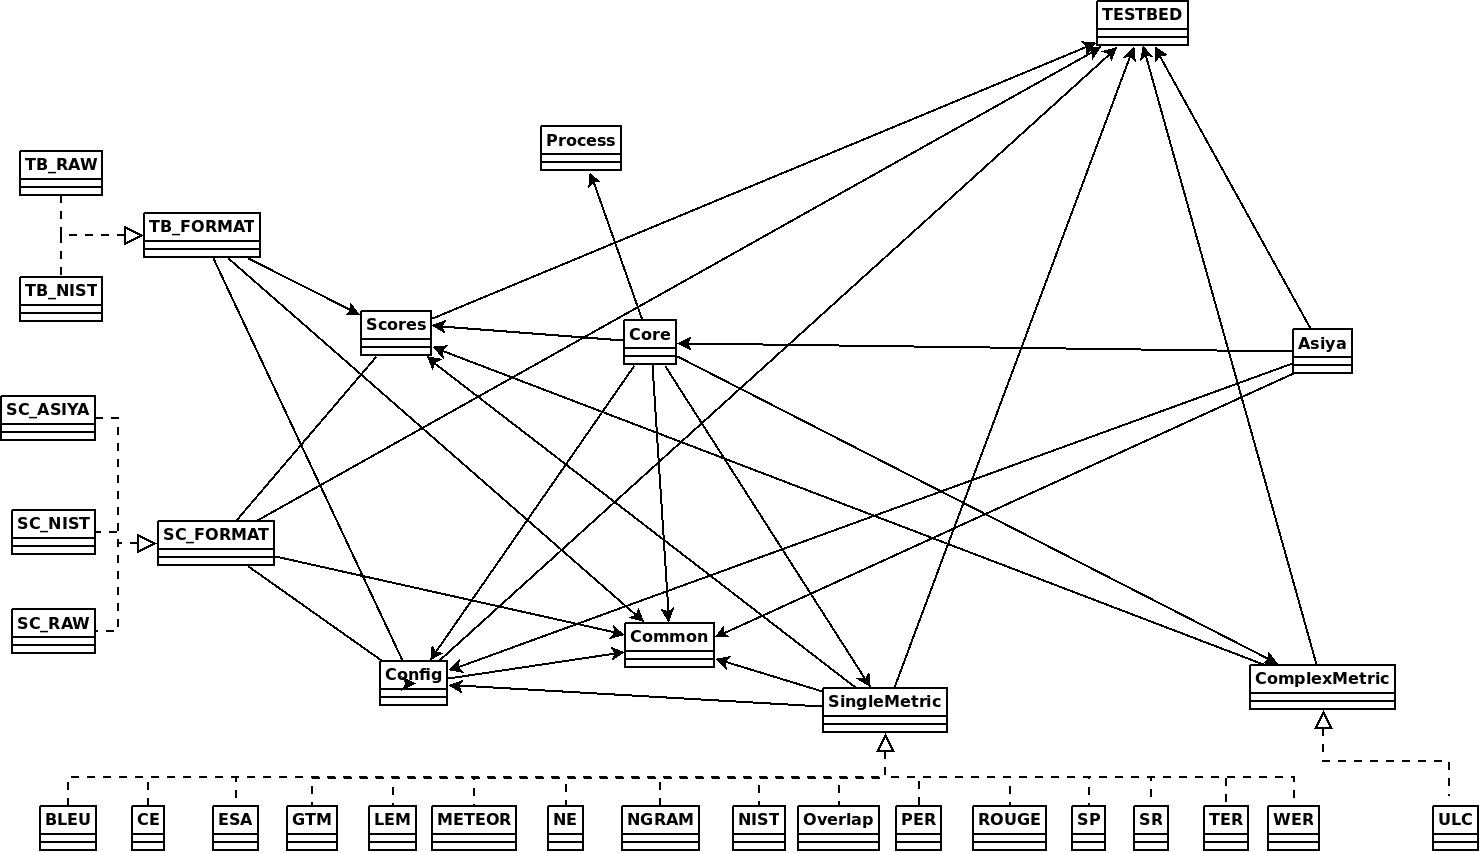
\includegraphics[width=1.2\textwidth]{resources/simple_diagram_v2.png}}
\caption{Diagrama de classes simplificat}
\end{figure}

Algunes d'aquestes classes ja formaven part de la versió d'\texttt{ASIYA} de la qual hem partit. Altres són fruit de la re-estructuració de tota l'eina amb funcionalitats que ja eren presents. També hi ha classes noves que implementen funcionalitats noves.
\\

Podem classificar totes aquestes classes conceptualment en els següents grups:
\begin{enumerate}
\item \textit{Nucli}: Podríem dir que s'encarreguen del \textit{pipeline} de l'aplicació. Aquestes classes són  \texttt{Asiya} i \texttt{Core}. Les dues són classes noves i resumeixen el funcionament de l'aplicació. Mentre que \texttt{Asiya} actua com a interfície d'usuari i parametritza l'execució de l'eina, \texttt{Core} és el nucli que actua de \textit{master} de la paral·lelització, encarregat de tota la gestió de l'avaluació.

\item \textit{Avaluació}: En formen part totes aquelles classes que tenen una significació de "mètrica" o "avaluació". Aquestes són tant \texttt{SingleMetric} com \texttt{ComplexMetric} i totes les classes que en deriven respectivament: les implementacions de cada família de mètriques d'avaluació. Aquestes últimes ja existien i són pures transcripcions. No obstant s'ha afegit les classes abstractes així com mètodes compartits, heretats i sobreescrits per a un disseny més coherent (secció 4.5).

\item \textit{Dades}: Integren aquest grup la classe \texttt{TESTBED}, la qual simbolitza el joc de proves amb el que operem -abstracció nova- i la classe \texttt{Scores}, la qual representa tot el contingut obtingut de les avaluacions.

\item \textit{Format}: Si bé és cert que part del contingut d'algunes classes ja existia, s'ha hagut de redissenyar tot i adaptar-lo al nou llenguatge. En formen part \texttt{TB\_FORMAT}, \texttt{SC\_FORMAT} i totes les classes derivades, respectivament. La secció 4.4 explica les seves principals característiques més detalladament.

\item \textit{Paral·lelisme} És la funcionalitat nova, que complementa la funcionalitat principal d'avaluació. La classe \texttt{Process} és l'encarregada de fer-ho possible.

\item \textit{Configuració}: Les constants del sistema i valors per defecte són els components de la classe \texttt{Common}. D'altra banda, la classe \texttt{Config} encapsula els paràmetres de configuració, i en definitiva tot el referent a la parametrització del sistema.
\end{enumerate}

Els canvis realitzats en el disseny original es resumeixen en la taula 1.

\begin{table}[H]
\makebox[\linewidth]{
\begin{tabular}{l  r}
\hline
Classe        & Reivisió       \\ [0.25ex]
\hline\hline
\texttt{Asiya}         & \textit{IGUAL} \\
\texttt{Core}          & \textit{NOVA}           \\
\texttt{SingleMetric}  & \textit{NOVA}           \\
\texttt{ComplexMetric} & \textit{NOVA}           \\
\texttt{BLEU}          & \textit{IGUAL}          \\
\texttt{CE}            & \textit{IGUAL}          \\
\texttt{ESA}           & \textit{IGUAL}          \\
\texttt{GTM}           & \textit{IGUAL}          \\
\texttt{LEM}           & \textit{IGUAL}          \\
\texttt{METEOR}        & \textit{IGUAL}               \\
\texttt{NE}            & \textit{IGUAL}               \\
\texttt{NGRAM}         & \textit{IGUAL}               \\
\texttt{NIST}          & \textit{IGUAL}               \\
\texttt{Overlap}       & \textit{IGUAL}               \\
\texttt{PER}           & \textit{IGUAL}               \\
\texttt{ROUGE}         & \textit{IGUAL}              \\
\texttt{SP}            & \textit{IGUAL}               \\
\texttt{SR}            & \textit{IGUAL}               \\
\texttt{TER}           & \textit{IGUAL}               \\
\texttt{WER}           & \textit{IGUAL}               \\
\texttt{ULC}           & \textit{IGUAL}               \\
\texttt{TESTBED}       & \textit{NOVA}           \\
\texttt{Scores}        & \textit{IGUAL}          \\
\texttt{TB\_FORMAT}    & \textit{NOVA}           \\
\texttt{TB\_RAW}       & \textit{REIMPLEMENTADA}           \\
\texttt{TB\_NIST}      & \textit{REIMPLEMENTADA}           \\
\texttt{SC\_FORMAT}    & \textit{NOVA}           \\
\texttt{SC\_ASIYA}     & \textit{REIMPLEMENTADA}           \\
\texttt{SC\_NIST}      & \textit{REIMPLEMENTADA}           \\
\texttt{SC\_RAW}       & \textit{REIMPLEMENTADA}               \\
\texttt{Process}       & \textit{NOVA}           \\
\texttt{Config}        & \textit{IGUAL}          \\
\texttt{Common}        & \textit{IGUAL}    		\\     
\hline
\end{tabular}}
\caption{Exemple fitxer \textit{report}}
\end{table}

L'estat ``Reimplementat'' indica que les funcionalitats de la classe no són noves però el disseny i l'estructura de la mateixa sí.

\subsection{Metodologia d'ús}
A més de l'\textit{input/output} d'\texttt{ASIYA} que hem definit a l'apartat 1.1, hi ha diverses opcions de configuració en l'execució d'\texttt{ASIYA}. Alguns d'aquestes opcions acompanyen a la crida al sistema en forma de paràmetres \textit{(flags)} en la línia de comandes.
\\

Els paràmetres més comuns:

\begin{itemize}
\item \texttt{-v}: \textit{verbose}.

\item \texttt{-h}: \textit{help}. Manual d'usuari.

\item \texttt{-time}: Comptabilitza el temps d'execució de cada mètrica.

\item \texttt{-metric\_set}: Referència al conjunt de mètriques a executar indicades en el fitxer de configuració (secció 4.3).

%\item \texttt{-system\_set}: \textit{verbose}.

%\item \texttt{-reference\_set}: \textit{verbose}.

\item \texttt{-g}: Granularitat dels resultats: \textit{score} per oració, document o sistema.

\item \texttt{-eval}: Tipus de mètriques d'avaluació (secció 4.4).

\item \texttt{-data\_path}: Ruta als fitxers.

\item \texttt{-paralel}: Indicador de paral·lelisme. Va seguit del nombre de particions desitjades.

%\item \texttt{-serialize}: Aquest paràmetre només està pensat per a l'ús intern d'\texttt{ASIYA} en l'execució dels subprocessos. Serveix de convertidor entre la posició de les oracions del subprocés (relativa) a la posició en el text original (absoluta).
\end{itemize}

Un exemple de crida amb paràmetres és el següent:

\begin{table}[H]
\makebox[\linewidth]{
\begin{tabular}{l}
\hline
\\
\texttt{./Asiya Asiya.config -time -v -eval single,ulc -g sys -metric\_set metrics\_SP} \\
\texttt{ -data\_path /home/usuaris/gilabert/RUN\_TEST > SP.report} \\
\\
\hline
\end{tabular}}
%\caption{Exemple d'execució d'\texttt{ASIYA}}
\end{table}



\subsection{Opcions de configuració}
A més dels atributs vistos en la secció anterior, hi ha més opcions a configurar. L'execució d'\texttt{ASIYA} ha d'anar acompanyada d'un fitxer de configuració \textit{(.config)}. En aquest fitxer, indicarem altres opcions com les llengües de les traduccions. A més, podem afegir algunes de les opcions vistes en la secció anterior per a millor confort.
\\

A continuació un exemple de fitxer de configuració:
\begin{table}[H]
\makebox[\linewidth]{
\begin{tabular}{l}
\hline
\\
\# lines starting with '\#' are ignored                                    \\
																		   \\
input=nist																   \\
																		   \\
srclang=es																   \\
srccase=cs																   \\
trglang=en																   \\
trgcase=cs																   \\
                                                                           \\
src=source.xml                                                             \\
sys=candidates.xml                                                         \\
ref=references.xml                                                         \\
                                                                           \\
some\_metrics=-TERp METEOR-pa CP-STM-6 DP-Or(*) SR-Or(*) DR-Or(*) DR-STM-6 \\
%some\_systems=system01 system05 system 07                                  \\
%some\_refs=reference02 reference04                                         \\
metrics\_rouge=ROUGE-1 ROUGE-2 ROUGE-3 ROUGE-4 ROUGE-L ROUGE-S*	 	       \\
\ \ \ \ \ \ \ \ \ \ \ \ \ \ \ \ \ \ \ \ ROUGE-SU* ROUGE-W 				   \\
\\
\hline
\end{tabular}}
%\caption{Exemple de fitxer de configuració $Asiya.config$}
\end{table}


Els paràmetres reconeguts en el fitxer de configuració són els següents:

\begin{itemize}
\item \texttt{input}: Format en el qual \texttt{ASIYA} espera trobar els fitxers \textit{src}, \textit{reference} i \textit{system} esmentats en la secció 1.1. La tipologia de formats es detalla en la següent secció.

\item \texttt{srclang}: Llengua origen de la traducció.

\item \texttt{srccase}: \textit{Case Sensitive} / \textit{Case Insensitive} de la llengua origen de la traducció.

\item \texttt{trglang}: Llengua destí de la traducció.

\item \texttt{trgcase}: \textit{Case Sensitive} / \textit{Case Insensitive} de la llengua destí de la traducció.

\item \texttt{src}/\texttt{source}: Text en la llengua origen de la traducció.

\item \texttt{ref}/\texttt{reference}: Conjunt de referències en la llengua destí.

\item \texttt{sys}/\texttt{system}: Conjunt de traduccions automàtiques a avaluar.

\item \texttt{metric\_set}: Defineix un conjunt de mètriques simples. Definim aquests conjunts de manera arbitrària per alleugerir la crida al sistema d'\texttt{ASIYA} (línia de comandes).
\end{itemize}


\subsection{Input/Output}

\texttt{ASIYA} accepta dos formats diferents. Per un costat el \texttt{txt} (text pla\cite{textfile}); i per l'altre \texttt{xml} [NIST XML especificat en el \textit{Metrics MaTr Evaluation Plan}\cite{nist_xml}].
\\

Aquests són els dos formats vàlids per als fitxers d'entrada. Degut a aquesta dualitat en la revisió del disseny vam definir les classes \textit{TB\_RAW} i \textit{TB\_NIST} les quals deriven de la classe abstracta \textit{TB\_FORMAT} referida als fitxers d'entrada del sistema. No obstant hi ha mètriques que requereixen certa personalització d'aquests formats. Tot el tractament intern del sistema i les particularitats d'algunes mètriques pel que fa a formatació també s'inclouen en aquestes classes.
\\

Així doncs, tot el que conceptualment té una significació de \textit{input} queda englobat en la classe \textit{TB\_FORMAT}, essent així una manera més ordenada d'entendre les dades.
\\

Anàlogament, per a tot allò que fa referència a l'\textit{output} i la formatació dels resultats s'ha dissenyat la classe \textit{SC\_FORMAT}, de la mateixa manera que \textit{TB\_FORMAT} en deriven \textit{SC\_RAW} i \textit{SC\_NIST} pels respectius formats. Aquestes classes contenen tot allò relacionat amb la maquetació i construcció de l'informe \textit{(report)} que genera \texttt{ASIYA} amb les puntuacions de cada mètrica, sistema, etc.
\\

La Taula 3 mostra un exemple d'informe. En aquest informe apareix l'avaluació realitzada sobre un conjunt de documents (columna ``SET'') de 5 sistemes de traducció automàtica (columna ``SYS''), i els valors d'avaluació obtinguts a través de 4 mètriques diferents (columnes ``GTM1'', ``GTM2'', ``GTM3'' i ``ULC'').
\\

\begin{table}[H]
\makebox[\linewidth]{
\begin{tabular}{l l r r r r}
\hline
SET                 & SYS     & GTM-1      & GTM-2      & GTM-3      & ULC        \\ [0.25ex]
\hline\hline
newssyscombtest2010 & onlineA & 0.52610169 & 0.23252133 & 0.19372313 & 0.90878835 \\
newssyscombtest2010 & onlineB & 0.56339959 & 0.25759535 & 0.21768959 & 1.00000000 \\
newssyscombtest2010 & uedin   & 0.54064772 & 0.24013189 & 0.20095511 & 0.93831651 \\
newssyscombtest2010 & upc     & 0.53403833 & 0.23256854 & 0.19331048 & 0.91291325 \\
newssyscombtest2010 & combo   & 0.54050465 & 0.24146659 & 0.20142303 & 0.94067548
\\ [0.5ex]
\hline
\end{tabular}}
%\caption{Exemple fitxer \textit{report}}
\end{table}

A més del \textit{report} esmentat, \texttt{ASIYA} emmagatzema els resultats de l'avaluació de cada mètrica(de manera arbòria per a cada sistema i referència) en un fitxer amb format \texttt{xml} comprimit. És fa d'aquesta manera amb la finalitat de no repetir càlculs en avaluacions similars d'execucions posteriors. Per aquest afegit es va confeccionar la classe \textit{SC\_ASIYA}, igualment hereva de \textit{SC\_FORMAT}.


\begin{table} [H]
\makebox[\linewidth]{
\begin{tabular}{l}
\hline
%\\
\textless?xml version="1.0" encoding=''UTF-8''?\textgreater  				        \\
\textless !DOCTYPE REPORT SYSTEM "asiya.dtd{[}{]}"\textgreater                      \\
\textless REPORT hyp="onlineA" metric="METEOR-ex" n\_docs="3" n\_segments="33" 		\\
\ \ \ \ \ \ \ \ \ \ \ \ \ \ \ \ \ \ \ \ \ \ \ \ \ ref="reference01" score="0.22711204"\textgreater \\
\ \ \ \ \ \textless DOC id="idnes.cz/2009/12/11/76492" n="1" n\_segments="10" score="0.18251989"\textgreater \\
\ \ \ \ \ \ \ \ \textless S n="1"\textgreater0.18067883\textless/S\textgreater \\
\ \ \ \ \ \ \ \ \textless S n="2"\textgreater0.10353373\textless/S\textgreater \\
\ \ \ \ \ \ \ \ \textless S n="3"\textgreater0.10322581\textless/S\textgreater \\
\ \ \ \ \ \ \ \ \textless S n="4"\textgreater0.23817324\textless/S\textgreater \\
\ \ \ \ \ \ \ \ \textless S n="5"\textgreater0.25554795\textless/S\textgreater \\
\ \ \ \ \ \ \ \ \textless S n="6"\textgreater0.15165877\textless/S\textgreater \\
\ \ \ \ \ \ \ \ \textless S n="7"\textgreater0.14773289\textless/S\textgreater \\
\ \ \ \ \ \ \ \ \textless S n="8"\textgreater0.22220717\textless/S\textgreater \\
\ \ \ \ \ \ \ \ \textless S n="9"\textgreater0.11616584\textless/S\textgreater \\
\ \ \ \ \ \ \ \ \textless S n="10"\textgreater0.25871569\textless/S\textgreater \\
\ \ \ \ \textless/DOC\textgreater \\
\ \ \ \ \textless DOC id="lidovky.cz/2009/12/10/75519" n="2" n\_segments="10" score="0.25064990"\textgreater \\
\ \ \ \ \ \ \ \ \textless S n="11"\textgreater0.26307932\textless/S\textgreater \\
\ \ \ \ \ \ \ \ \textless S n="12"\textgreater0.21008388\textless/S\textgreater \\
\ \ \ \ \ \ \ \ \textless S n="13"\textgreater0.23357930\textless/S\textgreater \\
\ \ \ \ \ \ \ \ \textless S n="14"\textgreater0.21300650\textless/S\textgreater \\
\ \ \ \ \ \ \ \ \textless S n="15"\textgreater0.38905645\textless/S\textgreater \\
\ \ \ \ \ \ \ \ \textless S n="16"\textgreater0.32702883\textless/S\textgreater \\
\ \ \ \ \ \ \ \ \textless S n="17"\textgreater0.15404394\textless/S\textgreater \\
\ \ \ \ \ \ \ \ \textless S n="18"\textgreater0.20456945\textless/S\textgreater \\
\ \ \ \ \ \ \ \ \textless S n="19"\textgreater0.14927177\textless/S\textgreater \\
\ \ \ \ \ \ \ \ \textless S n="20"\textgreater0.33922408\textless/S\textgreater \\
\ \ \ \ \textless/DOC\textgreater \\
\ \ \ \ \textless DOC id="lidovky.cz/2009/12/10/75501" n="3" n\_segments="13" score="0.23568691"\textgreater \\
\ \ \ \ \ \ \ \ \textless S n="21"\textgreater0.23926208\textless/S\textgreater \\
\ \ \ \ \ \ \ \ \textless S n="22"\textgreater0.47107745\textless/S\textgreater \\
\ \ \ \ \ \ \ \ \textless S n="23"\textgreater0.27414713\textless/S\textgreater \\
\ \ \ \ \ \ \ \ \textless S n="24"\textgreater1.00000000\textless/S\textgreater \\
\ \ \ \ \ \ \ \ \textless S n="25"\textgreater0.15101167\textless/S\textgreater \\
\ \ \ \ \ \ \ \ \textless S n="26"\textgreater0.14303702\textless/S\textgreater \\
\ \ \ \ \ \ \ \ \textless S n="27"\textgreater0.19645855\textless/S\textgreater \\
\ \ \ \ \ \ \ \ \textless S n="28"\textgreater0.24086132\textless/S\textgreater \\
\ \ \ \ \ \ \ \ \textless S n="29"\textgreater0.27986060\textless/S\textgreater \\
\ \ \ \ \ \ \ \ \textless S n="30"\textgreater0.32660807\textless/S\textgreater \\
\ \ \ \ \ \ \ \ \textless S n="31"\textgreater0.26293743\textless/S\textgreater \\
\ \ \ \ \ \ \ \ \textless S n="32"\textgreater0.29977810\textless/S\textgreater \\
\ \ \ \ \ \ \ \ \textless S n="33"\textgreater0.17493735\textless/S\textgreater \\
\ \ \ \ \textless/DOC\textgreater \\
\textless/REPORT\textgreater \\
%\\                          
\hline
\end{tabular} }
\begin{quote}
\centering
Exemple fitxer de \textit{scores} \texttt{XML}
\end{quote}
%\caption{Exemple fitxer de \textit{scores} \texttt{XML}}
\end{table}

\subsection{Opcions d'avaluació}

Com es cita en seccions anteriors, en la configuració d'\texttt{ASIYA} s'indica el tipus d'avaluació que desitgem mitjançant l'opció \texttt{-eval}; amb aquesta opció es determina quin tipus de mètriques s'avaluaran. Hem de diferenciar dos tipus.

\paragraph{\textit{Single Metric}:} Mètrica simple o homogènia. És una abstracció per agrupar totes aquelles mètriques autoconclosives. És a dir, sense cap dependència en temps d'execució. Cadascuna genera un \textit{score}. La majoria de les mètriques actuals formen part d'aquest conjunt.
\\

%\textit{(BLEU BLEU-1 BLEU-2 BLEU-3 BLEU-4 BLEUi-2 BLEUi-3 BLEUi-4)}
%\textit{(NIST NIST-1 NIST-2 NIST-3 NIST-4 NIST-5 NISTi-2 NISTi-3 NISTi-4 NISTi-5)}
Totes aquestes mètriques són paral·lelitzables excepte les de la família \texttt{BLEU} i les de la família \texttt{NIST}. Això és degut a que el càlcul del \textit{score} a nivell de document és més sofisticat que la mitjana aritmètica dels \textit{scores} de les oracions (mètode usat per altres famílies de mètriques). Per tant, no és poden avaluar les oracions de manera independent.

\paragraph{\textit{Complex Metric}:} Mètrica composta o heterogènia. És una abstracció per agrupar totes aquelles mètriques que sí són dependents d'altres. Les d'aquest tipus requereixen l'avaluació prèvia de les mètriques simples.
\\

Actualment hi ha disponible una sola mètrica d'aquesta tipologia:

\begin{itemize}
\item \textbf{Ulc}: Mitjana aritmètica normalitzada dels \textit{scores}.
\end{itemize}

Per exemple:

\begin{quote}
\texttt{./Asiya Asiya.config -v -eval single,ulc -metric\_set metrics\_BLEU}
\end{quote}

Calcularà els \textit{scores} de cada mètrica simple del conjunt \texttt{metrics\_BLEU} definit en el fitxer de configuració i la seva mitjana aritmètica normalitzada.
\\

A més de l'informe d'avaluació (taula 3) \texttt{ASIYA} genera els resultats de l'execució de les mètriques en el directori \texttt{"./scores/"} a fi de no re-calcular traduccions ja avaluades (taula 4). No obstant, podem forçar la re-avaluació amb l'opció \texttt{-remake}.
\\

En el manual d'\texttt{ASIYA} es pot trobar una descripció detallada de cada sistema d'avaluació\cite{asiya_manual}.


%\subsection{\texttt{ASIYA} \textit{Core}}
%No sé gaire què dir aquí.

%\subsection{\textit{Pipeline NLP}}
%Copy + Paste
\subsection{Processadors lingüístics}

Hi ha determinades mètriques on l'avaluació no es realitza sobre el text directament sinó que requereixen un preprocessament previ de les dades. D'aquests tractaments en resulten estructures lingüístiques a partir de les qual es realitzen els processos d'avaluació.
\\

A continuació detallarem breument alguns d'aquests processos en els quals podem identificar 2 grups:

\paragraph{\textbf{Processos a nivell de paraula}:}

\begin{itemize}
\item \textit{Lematització}: Procés pel qual s'obtenen les entrades diccionarials (lemes) que apareixen en un text sense tenir en compte l'estructura gramatical de la llengua. 
\\

Exemple:
\begin{quote}
``Your cats will eat fish'' $\longrightarrow$ ``your'' ``cat'' ``be'' ``eat'' ``fish''
\end{quote}

\item \textit{PoS tagging}: Procés de desambiguació pel qual s'etiqueta cada paraula d'un text amb la seva categoria morfosintàctica \textit{(Part of Speech -PoS-)} correcta segons el context de la paraula.
\\

Exemple:
\begin{quote}
``Your cats will eat fish'' $\longrightarrow$  ``fish'' (Pot ser \texttt{Nom\_Comu} o \texttt{Verb}, però en el context de l'oració es \texttt{Nom\_comu}).
\end{quote}
\end{itemize}


\paragraph{\textbf{Processos a nivell d'oració}:}
\begin{itemize}
\item \textit{Anàlisi sintàctica} \textit{(Syntactic Parsing)} -també existeix \textit{Semantic Parsing}, per a més informació consultar el manual d'\texttt{ASIYA}\cite{asiya_manual}-: Procés pel qual s'obté una representació més o menys profunda de l'estructura sintàctica que subsumeix l'oració.

\item \textit{Chunking}: És una anàlisi sintàctica superficial, amb la qual l'estructura sintàctica de l'oració es representa a través de la seqüencia de \textit{constituent sintàctics (chunk)} que hi participen, deixant de banda les funcions sintàctiques (com ara subjecte, objecte directe,...) que els relacionen.
\\

Exemple:
\begin{quote}
``Your cats will eat fish'' $\longrightarrow$ (SN Your cat) (SV will eat) (SN fish)
\end{quote}

\item \textit{Head} (Nucli): És la paraula amb el significat principal dins d'un constituent sintàctic.
\\

Exemple:
\begin{quote}
(SN Your cat) $\longrightarrow$ $head=cat$
\end{quote}

\end{itemize}





\subsection{Alternatives}
Com es comenta en la secció 2.1.1 en un estadi inicial es plantejava la possibilitat d'adaptar la nova versió del sistema en una arquitectura de computació paral·lela estil GPGPU \textit{(General-Purpose Computing on Graphics Processing Units)}. Tot i que aquest paradigma prometia molt s'ha descartat per la poca versatilitat que ofereix. El model \textit{GPU computing} brinda molta ``força bruta'' pel que fa a càlcul estrictament parlant. D'altra banda, la poca o nul·la interrelació de les diferents mètriques -la compartició de memòria és fonamental en execucions eficients en GPUs- i la dispersa tipologia de les mateixes -implementades en llenguatges diferents- ens obliguen a optar per un esquema de propòsit general. 

\subsection{Llibreries de tercers}
Per a resoldre les mancances i contratemps que hem trobat durant tot el procés de desenvolupament, també s'ha hagut de fer ús de llibreries de tercers. Són de menester ja que el llenguatge no les proporciona per defecte. Per exemple, \textit{boost}\cite{boost} per a l'ús d'expressions regulars i tractament de fitxers a nivell de sistema operatiu; o un altre exemple més tangible, un \textit{parser} en \texttt{C++} per manipular fitxers en format XML -usat en les classes dedicades al format, citades en la secció 4.4-. L'escollit, principalment per la seva lleugeresa, és el  \textit{libxml}\cite{libxml}.



% % % % % % % % % % % % % % % % % % % % % % % % % % % % % % % % % % % % % % %
% % % % % % % % % % % % % % % % % % % % % % % % % % % % % % % % % % % % %
% % % % % % % % % % % % % % % % % % % % % % % % % % % % % % % % % % % % %
% % % % % % % % % % % % % % % % % % % % % % % % % % % % % % % % % % % % %
% % % % % % % % % % % % % % % % % % % % % % % % % % % % % % % % % % % % %
\newpage
\section{Experimentació}
En aquest apartat podrem mesurar l'impacte real que ha tingut el projecte i la millora aconseguida respecte la implementació d'\texttt{ASIYA} en \texttt{Perl}, que prenem com a \textit{baseline}.
\\

L'experimentació es dividirà en dos tipus d'experiments en els quals podrem comprovar diferents facetes del comportament de les diferents implementacions.
\\

\paragraph{Experiment 1} En aquest experiment es pretén comparar la versió seqüencial de la nova implementació en \texttt{C++} respecte la \textit{baseline} en \texttt{PERL} a fi de veure l'impacte produït només pel canvi de llenguatge (secció 5.1).
\\

Per dur a terme aquest experiment utilitzarem 5 corpus diferents.
\begin{itemize}
%\item \textit{ws\_corpus\_nist}: És el corpus més petit, conté 33 línies agrupades en 3 documents diferents. També és l'únic en format \texttt{xml}.

\item \textit{ws\_corpus100}: Corpus en format \texttt{txt}, conté 100 línies.

\item \textit{ws\_corpus200}: Corpus en format \texttt{txt}, conté 200 línies.

\item \textit{ws\_corpus500}: Corpus en format \texttt{txt}, conté 500 línies.

\item \textit{ws\_corpus1000}: Corpus en format \texttt{txt}, conté 1000 línies.

\item \textit{ws\_corpus2000}: Corpus en format \texttt{txt}, conté 2000 línies.

\end{itemize}


\paragraph{Experiment 2} En aquest experiment volem veure quin és el comportament de la nova versió d'\texttt{ASIYA} pel que fa al paral·lelisme, com escala en nombre de processos. Per dur-ho a terme hem escollit el corpus  \textit{ws\_corpus500}, ja que actua de mediana respecte la mida dels corpus que tenim a disposició (500 línies).
\\

\subsection{\texttt{C++} \emph{Vs.} \texttt{PERL}}
Com s'ha comentat anteriorment en aquests experiment compararem els temps d'execució de l'\texttt{ASIYA} original, implementada en \texttt{PERL} amb la nova versió d'\texttt{ASIYA} en C++; executada en mode seqüencial.
\\

En els següents apartats es mostren els resultats agrupats per a cada corpus: el nombre de sistemes a calcular i el temps emprat en cada implementació, respectivament.

\begin{comment}
%\newpage
\subsubsection{\emph{ws\_corpus\_nist}}
%%%%%%%%%%%%%%%%%
%%% ws_corpus_nist
%%%%%%%%%%%%%%%%%
\begin{table}[h]
\centering
\caption{\textit{ws\_corpus\_nist}}
\begin{tabular}{l r r | r r | r r}
\hline\hline 
       & \multicolumn{2}{c}{1 system} & \multicolumn{2}{c}{3 systems} & \multicolumn{2}{c}{5 systems} \\ [0.25ex] \hline
Metric & \texttt{PERL}          & \texttt{C++}          & \texttt{PERL}           & \texttt{C++}          & \texttt{PERL}          & \texttt{C++} \\ [0.25ex] \hline \hline
SP     & 15,15         & 16,04        & 33,38         & 35,87         & 62,15         & 57,25         \\
SR     & 62,98         & 64,79        & 134,18        & 140,78        & 209,30        & 216,19        \\
CE     & 21,32         & 21,53        & 41,57         & 41,23         & 69,64         & 61,95         \\
ESA    & 3,03          & 4,28         & 8,18          & 9,42          & 13,68         & 16,45         \\
GTM    & 0,56          & 1,20         & 1,71          & 3,16          & 2,91          & 5,26          \\
LEM    & 0,43          & 0,96         & 1,36          & 2,50          & 3,49          & 3,99          \\
METEOR & 15,90         & 17,87        & 47,87         & 49,03         & 82,02         & 83,52         \\
NE     & 0,31          & 0,74         & 0,96          & 2,01          & 3,04          & 3,52          \\
NGRAM  & 3,35          & 4,27         & 10,05         & 10,98         & 18,11         & 19,78         \\
O      & 0,00          & 0,12         & 0,01          & 0,33          & 0,02          & 0,55          \\
PER    & 0,07          & 0,30         & 0,19          & 0,87          & 0,62          & 1,43          \\
ROUGE  & 1,01          & 2,18         & 3,03          & 6,44          & 9,64          & 10,77         \\
TER    & 40,38         & 60,07        & 123,09        & 140,05        & 224,39        & 285,71        \\
WER    & 0,20          & 0,44         & 0,61          & 1,28          & 1,94          & 2,17         \\ \hline
\end{tabular}
\label{table:Ex1-ws_corpus_nist}
\end{table}
\end{comment}


\newpage
\subsubsection{Resultats}
%\begin{landscape}
%\newpage
%\subsubsection{\emph{ws\_corpus100}}
%%%%%%%%%%%%%%%%%
%%% ws_corpus100
%%%%%%%%%%%%%%%%%
\begin{table}[H]
\centering
\caption{Temps d'execució (\textit{s}) del corpus \textit{ws\_corpus100}}
\footnotesize
\makebox[\linewidth]{
\begin{tabular}{l r r | r r | r r | r r | r r }
\hline\hline 
       & \multicolumn{2}{c}{1 system} & \multicolumn{2}{c}{2 systems} & \multicolumn{2}{c}{5 systems} & \multicolumn{2}{c}{10 systems} & \multicolumn{2}{c}{14 systems} \\ [0.5ex] \hline
Metric & \texttt{PERL}          & \texttt{C++}          & \texttt{PERL}           & \texttt{C++}          & \texttt{PERL}          & \texttt{C++}           & \texttt{PERL}           & \texttt{C++}           & \texttt{PERL}           & \texttt{C++}           \\ [0.25ex] \hline \hline
SP     & 26,70         & 26,24        & 36,35          & 40,18        & 82,37         & 85,07         & 147,46         & 104,72        & 203,33         & 118,96        \\
SR     & 1002,24       & 747,24       & 1136,67        & 796,55       & 1732,69       & 1098,17       & 2526,05        & 1735,59       & 2260,71        & 2098,48       \\
CE     & 26,13         & 28,06        & 37,68          & 37,67        & 75,05         & 65,50         & 147,76         & 100,63        & 200,78         & 142,27        \\
ESA    & 5,89          & 39,16        & 11,65          & 15,26        & 31,07         & 37,25         & 62,35          & 63,67         & 108,37         & 88,14         \\
GTM    & 0,85          & 1,05         & 1,70           & 2,84         & 4,44          & 6,76          & 9,67           & 12,29         & 18,91          & 16,85         \\
LEM    & 0,58          & 0,87         & 1,19           & 1,98         & 3,08          & 4,41          & 6,18           & 8,67          & 9,03           & 13,16         \\
METEOR & 17,02         & 18,55        & 34,38          & 32,58        & 85,93         & 85,94         & 172,49         & 171,49        & 297,76         & 241,25        \\
NE     & 0,75          & 0,81         & 1,52           & 1,40         & 3,98          & 4,84          & 8,14           & 9,74          & 11,48          & 13,42         \\
NGRAM  & 5,62          & 6,85         & 11,59          & 10,73        & 32,27         & 30,48         & 56,93          & 60,10         & 104,50         & 84,06         \\
O      & 0,13          & 0,20         & 0,26           & 0,28         & 0,65          & 1,24          & 1,17           & 2,45          & 1,61           & 3,53          \\
PER    & 0,10          & 0,32         & 0,19           & 0,40         & 0,43          & 1,70          & 0,90           & 3,42          & 1,21           & 4,75          \\
ROUGE  & 3,30          & 5,29         & 6,62           & 8,14         & 16,66         & 31,28         & 37,57          & 61,85         & 47,42          & 85,55         \\
TER    & 88,82         & 151,41       & 171,39         & 172,23       & 478,91        & 465,68        & 863,41         & 930,91        & 1198,30        & 1303,21       \\
WER    & 0,52          & 0,66         & 0,99           & 1,06         & 2,51          & 4,19          & 5,17           & 7,40          & 7,45           & 11,02			\\ \hline
\end{tabular}}
\label{table:Ex1-ws_corpus100}
\normalsize
\end{table}
%\end{landscape}

%\newpage
%\subsubsection{\emph{ws\_corpus200}}
%%%%%%%%%%%%%%%%%
%%% ws_corpus200
%%%%%%%%%%%%%%%%%
\begin{table}[H]
\centering
\caption{Temps d'execució (\textit{s}) del corpus \textit{ws\_corpus200}}
\footnotesize
\makebox[\linewidth]{
\begin{tabular}{l r r | r r | r r | r r | r r }
\hline\hline 
       & \multicolumn{2}{c}{1 system} & \multicolumn{2}{c}{2 systems} & \multicolumn{2}{c}{5 systems} & \multicolumn{2}{c}{10 systems} & \multicolumn{2}{c}{14 systems} \\ [0.5ex] \hline
Metric & \texttt{PERL}          & \texttt{C++}          & \texttt{PERL}          & \texttt{C++}           & \texttt{PERL}          & \texttt{C++}           & \texttt{PERL}           & \texttt{C++}           & \texttt{PERL}           & \texttt{C++}           \\ [0.25ex] \hline \hline
SP     & 29,53         & 34,82        & 48,17         & 53,73         & 107,82        & 110,78        & 196,04         & 140,38        & 270,45         & 154,13        \\
SR     & 1402,55       & 1217,89      & 2054,18       & 1385,12       & 2722,90       & 1913,16       & 3178,69        & 3653,28       & 3782,32        & 4418,58       \\
CE     & 28,43         & 27,57        & 46,94         & 39,56         & 96,45         & 70,86         & 145,80         & 104,84        & 212,51         & 145,54        \\
ESA    & 10,45         & 16,17        & 19,70         & 21,80         & 60,20         & 58,70         & 106,54         & 106,49        & 147,71         & 182,06        \\
GTM    & 1,40          & 1,57         & 2,45          & 3,11          & 8,16          & 7,74          & 13,78          & 14,27         & 16,27          & 19,91         \\
LEM    & 0,61          & 1,06         & 1,25          & 2,10          & 3,24          & 5,02          & 6,41           & 9,78          & 8,12           & 11,79         \\
METEOR & 18,43         & 18,44        & 38,10         & 35,53         & 97,50         & 90,60         & 184,31         & 181,91        & 264,73         & 252,83        \\
NE     & 1,91          & 1,11         & 2,57          & 2,35          & 6,68          & 6,08          & 20,80          & 11,98         & 17,58          & 17,63         \\
NGRAM  & 8,79          & 8,25         & 17,59         & 16,56         & 55,30         & 42,52         & 87,69          & 83,31         & 149,54         & 118,13        \\
O      & 0,35          & 0,40         & 0,44          & 0,82          & 1,09          & 2,04          & 3,25           & 4,15          & 3,20           & 5,76          \\
PER    & 0,09          & 0,39         & 0,22          & 0,80          & 0,51          & 1,95          & 1,40           & 3,98          & 1,53           & 5,52          \\
ROUGE  & 9,32          & 11,09        & 12,84         & 23,58         & 31,57         & 58,96         & 99,33          & 116,73        & 89,67          & 166,70        \\
TER    & 125,23        & 156,16       & 262,57        & 263,55        & 565,92        & 663,63        & 1277,58        & 1381,82       & 1852,25        & 2008,63       \\
WER    & 0,95          & 1,51         & 1,72          & 2,54          & 4,38          & 6,07          & 8,23           & 12,19         & 12,44          & 14,25        \\ \hline
\end{tabular}}
\label{table:Ex1-ws_corpus200}
\normalsize
\end{table}


%\newpage
%\subsubsection{\emph{ws\_corpus500}}
%%%%%%%%%%%%%%%%%
%%% ws_corpus500
%%%%%%%%%%%%%%%%%
\begin{table}[H]
\centering
\caption{Temps d'execució (\textit{s}) del corpus \textit{ws\_corpus500}}
\footnotesize
\makebox[\linewidth]{
\begin{tabular}{l r r | r r | r r | r r | r r }
\hline\hline
	& \multicolumn{2}{c}{1 system} & \multicolumn{2}{c}{2 systems} & \multicolumn{2}{c}{5 systems} & \multicolumn{2}{c}{10 systems} & \multicolumn{2}{c}{14 systems} \\ [0.5ex] \hline
Metric & \texttt{PERL}          & \texttt{C++}          & \texttt{PERL}          & \texttt{C++}           & \texttt{PERL}          & \texttt{C++}           & \texttt{PERL}           & \texttt{C++}           & \texttt{PERL}           & \texttt{C++}           \\ [0.25ex] \hline \hline
SP     & 48,97         & 60,04        & 76,61         & 98,59         & 173,38        & 185,13        & 361,35         & 367,55        & 402,92         & 467,79        \\
SR     & 4045,88       & 2670,64      & 4375,74       & 3709,35       & 4842,51       & 4898,22       & 10239,73       & 7677,59       & 8606,65        & 8847,41       \\
CE     & 44,39         & 36,66        & 52,90         & 51,66         & 101,97        & 80,51         & 208,52         & 145,90        & 229,26         & 201,16        \\
ESA    & 27,21         & 25,68        & 43,26         & 57,59         & 116,22        & 122,83        & 244,61         & 257,18        & 316,64         & 363,27        \\
GTM    & 2,78          & 2,17         & 4,06          & 4,49          & 10,40         & 10,59         & 26,54          & 18,30         & 43,67          & 24,92         \\
LEM    & 0,92          & 1,18         & 1,40          & 2,33          & 3,62          & 5,23          & 9,40           & 8,45          & 17,15          & 10,27         \\
METEOR & 28,75         & 21,78        & 39,85         & 46,66         & 107,77        & 112,68        & 293,29         & 221,10        & 369,58         & 318,88        \\
NE     & 2,95          & 1,66         & 6,12          & 3,85          & 14,08         & 9,08          & 31,14          & 18,68         & 61,91          & 18,71         \\
NGRAM  & 18,06         & 13,78        & 29,41         & 29,85         & 75,49         & 74,61         & 164,02         & 138,74        & 243,92         & 200,94        \\
O      & 0,48          & 0,81         & 1,10          & 1,67          & 2,39          & 3,44          & 5,14           & 6,45          & 6,54           & 6,68          \\
PER    & 0,17          & 0,57         & 0,34          & 1,11          & 0,79          & 2,69          & 1,64           & 5,28          & 2,88           & 6,62          \\
ROUGE  & 19,10         & 28,95        & 43,94         & 55,81         & 86,78         & 128,28        & 182,88         & 263,23        & 384,20         & 282,45        \\
TER    & 247,54        & 249,82       & 430,54        & 524,79        & 1086,27       & 1050,37       & 2442,56        & 2702,97       & 3223,96        & 3243,79       \\
WER    & 1,65          & 2,34         & 3,30          & 4,68          & 8,46          & 10,56         & 19,20          & 18,00         & 27,87          & 30,36        \\
\hline
\end{tabular}}
\label{table:Ex1-ws_corpus500}
\normalsize
\end{table}


%\newpage
%\subsubsection{\emph{ws\_corpus1000}}
%%%%%%%%%%%%%%%%%
%%% ws_corpus1000
%%%%%%%%%%%%%%%%%
\begin{table}[H]
\centering
\caption{Temps d'execució (\textit{s}) del corpus \textit{ws\_corpus1000}}
\footnotesize
\makebox[\linewidth]{
\begin{tabular}{l r r | r r | r r | r r | r r }
\hline\hline 
	& \multicolumn{2}{c}{1 system} & \multicolumn{2}{c}{2 systems} & \multicolumn{2}{c}{5 systems} & \multicolumn{2}{c}{10 systems} & \multicolumn{2}{c}{14 systems} \\ [0.5ex] \hline
Metric & \texttt{PERL}          & \texttt{C++}          & \texttt{PERL}          & \texttt{C++}           & \texttt{PERL}          & \texttt{C++}           & \texttt{PERL}           & \texttt{C++}           & \texttt{PERL}           & \texttt{C++}           \\ [0.25ex] \hline \hline
SP     & 91,52         & 108,39       & 136,54        & 162,86        & 299,80        & 330,73        & 572,04         & 644,84        & 881,65         & 870,32        \\
SR     & 8926,25       & 6694,70      & 7446,55       & 8092,93       & 10338,95      & 10845,15      & 21888,25       & 16207,13      & 20320,74       & 20218,00      \\
CE     & 57,16         & 52,00        & 69,62         & 65,76         & 148,96        & 109,67        & 243,35         & 177,55        & 345,19         & 228,39        \\
ESA    & 51,33         & 41,39        & 78,97         & 86,09         & 221,93        & 228,39        & 410,04         & 458,57        & 571,37         & 642,98        \\
GTM    & 2,95          & 2,53         & 5,43          & 5,14          & 15,23         & 12,17         & 26,34          & 29,39         & 34,41          & 35,17         \\
LEM    & 0,86          & 1,43         & 1,62          & 2,58          & 4,52          & 6,39          & 7,98           & 12,02         & 10,84          & 16,40         \\
METEOR & 23,99         & 24,42        & 45,04         & 48,25         & 123,81        & 129,20        & 212,81         & 255,44        & 281,73         & 353,39        \\
NE     & 5,11          & 2,62         & 10,97         & 5,45          & 27,34         & 14,74         & 48,02          & 30,61         & 66,55          & 41,16         \\
NGRAM  & 25,18         & 22,70        & 47,84         & 45,88         & 133,72        & 123,73        & 241,24         & 245,52        & 325,88         & 342,09        \\
O      & 0,91          & 1,56         & 1,86          & 2,85          & 4,67          & 6,30          & 8,54           & 12,07         & 11,55          & 16,99         \\
PER    & 0,25          & 0,79         & 0,50          & 1,48          & 1,23          & 3,36          & 2,19           & 6,43          & 3,01           & 8,40          \\
ROUGE  & 35,98         & 50,51        & 87,38         & 103,76        & 162,72        & 268,72        & 287,48         & 537,10        & 397,37         & 718,33        \\
TER    & 331,99        & 330,60       & 636,70        & 649,59        & 1769,84       & 1860,60       & 3329,15        & 3721,38       & 4353,38        & 5159,33       \\
WER    & 3,45          & 3,88         & 7,27          & 7,80          & 17,95         & 19,57         & 34,73          & 39,69         & 42,77          & 55,07        \\ \hline
\end{tabular}}
\label{table:Ex1-ws_corpus1000}
\normalsize
\end{table}


%\newpage
%\subsubsection{\emph{ws\_corpus2000}}
%%%%%%%%%%%%%%%%%
%%% ws_corpus2000
%%%%%%%%%%%%%%%%%
\begin{table}[H]
\centering
\caption{Temps d'execució (\textit{s}) del corpus \textit{ws\_corpus2000}}
\footnotesize
\makebox[\linewidth]{
\begin{tabular}{l r r | r r | r r | r r | r r }
\hline\hline 
	& \multicolumn{2}{c}{1 system} & \multicolumn{2}{c}{2 systems} & \multicolumn{2}{c}{5 systems} & \multicolumn{2}{c}{10 systems} & \multicolumn{2}{c}{14 systems} \\ [0.5ex] \hline
Metric & \texttt{PERL}          & \texttt{C++}          & \texttt{PERL}          & \texttt{C++}           & \texttt{PERL}          & \texttt{C++}           & \texttt{PERL}           & \texttt{C++}           & \texttt{PERL}           & \texttt{C++}           \\ [0.25ex] \hline \hline
SP     & 153,00   & 209,51   & 257,68    & 313,47   & 563,91    & 665,84   & 1108,64    & 1164,01  & 1535,44    & 1572,94  \\
SR     & 13242,36 & 13853,64 & 14945,96  & 15466,39 & 22185,55  & 22452,22 & 29870,90   & 30811,99 & 37953,12   & 38082,85 \\
CE     & 75,87    & 85,14    & 107,43    & 100,77   & 200,00    & 147,58   & 379,15     & 246,79   & 527,41     & 280,85   \\
ESA    & 68,90    & 72,53    & 160,57    & 163,08   & 409,73    & 421,37   & 915,49     & 905,54   & 1188,21    & 1216,75  \\
GTM    & 4,85     & 3,03     & 9,29      & 6,23     & 21,80     & 16,35    & 45,87      & 32,31    & 64,64      & 45,66    \\
LEM    & 1,40     & 1,77     & 2,89      & 3,06     & 6,78      & 7,39     & 13,51      & 14,46    & 19,32      & 19,97    \\
METEOR & 26,12    & 24,21    & 55,42     & 51,01    & 133,33    & 127,92   & 277,41     & 258,94   & 395,60     & 342,33   \\
NE     & 11,97    & 4,64     & 25,13     & 8,56     & 55,24     & 22,35    & 132,75     & 47,72    & 185,81     & 65,00    \\
NGRAM  & 44,38    & 43,46    & 87,53     & 84,92    & 222,35    & 217,61   & 439,96     & 440,18   & 618,29     & 561,69   \\
O      & 0,00     & 2,20     & 0,00      & 4,38     & 0,02      & 11,18    & 0,01       & 21,89    & 0,02       & 31,37    \\
PER    & 0,35     & 1,24     & 1,21      & 2,19     & 2,76      & 4,74     & 5,56       & 9,82     & 7,36       & 13,24    \\
ROUGE  & 88,29    & 106,03   & 176,71    & 198,20   & 456,11    & 487,07   & 931,35     & 1055,28  & 1332,24    & 1408,96  \\
TER    & 440,89   & 513,06   & 864,11    & 998,77   & 2217,26   & 2509,01  & 4350,85    & 5170,91  & 6070,81    & 6577,34  \\
WER    & 7,12     & 7,58     & 14,26     & 14,92    & 34,73     & 36,56    & 69,46      & 77,16    & 97,39      & 96,68    \\ \hline
\end{tabular}}
\label{table:Ex1-ws_corpus2000}
\normalsize
\end{table}


\afterpage{\clearpage}
\subsubsection{Conclusions}
En aquest experiment hem pogut veure l'impacte que té la tria de llenguatge en la implementació del sistema. No sembla un canvi molt significatiu a primer cop d'ull, i és que cal recordar que les implementacions de les mètriques són de naturalesa molt diversa i encara que \texttt{ASIYA} ara sigui un programa en \texttt{C++}, com ja es va comentar en el Context del projecte cada mètrica és diferent i inaccessible.
\\

Podem observar com hi ha mètriques amb una millora notable i d'altres amb mesuraments similars o fins i tot pitjors. Tot i que a priori podríem pensar en una millora més pronunciada atribuïm la similitud dels resultats a la implementació interna de cadascuna de les mètriques provades. Pel que fa a les desviacions negatives, en la secció 4.7 parlàvem de la necessitat d'incloure programació de tercers. Cal destacar que això juga a favor de \texttt{PERL} ja que ha demostrat (comprovat en experiments paral·lels) la seva superioritat en el tractament d'expressions regulars.
\\

Pel que fa a mida del joc de proves, sembla que escala de manera propera a la linealitat.
\\

També cal recordar que l'execució d'aquest experiment està subjecte al \textit{hardware} de cada node del \textit{cluster} (secció 2.1.2). Depenent de l'antiguitat del node pot haver diferències molt considerables pel que fa a potència de càlcul.
\\

Si entrem a valorar amb més detall els resultats obtinguts podem fer una abstracció i agrupar-los en 3 conjunts no disjunts segons el comportament de cada mètrica. Aquestes grups són: 

\begin{itemize}
\item \textit{Independència dels paràmetres}: Són el cas de \textit{ESA} o \textit{WER}, on es pot veure la mateixa tendència independent de la mida dels text, el nombre de sistemes i les diferents implementacions, ambdues mostren un cost lineal respecte el nombre de sistemes a avaluar. Les petites desviacions no es poden atribuir a un canvi en el comportament de l'algorisme.


\item \textit{Dependència del nombre de sistemes}: Les mètriques \textit{CE}, \textit{METEOR} i \textit{NGRAM} mostren una clara millora en el seu comportament a mesura que augmenten el nombre de sistemes donat un corpus. Ens podem fixar, per exemple, en la mètrica \textit{CE}: donat 1 sistema, per a tots els corpus triga aproximadament el mateix en les dues implementacions (\texttt{PERL}/\texttt{C++}). En canvi, per a tots els sistemes (14) la versió en \texttt{C++} és 1,4 vegades més ràpida que l'equivalent en \texttt{PERL} per a tots els cassos i assolint un \textit{speed up} de 1,87 en el corpus més gran.


\item \textit{Dependència de la mida del corpus}: Ens podem fixar com hi ha mètriques com \textit{SP} on el canvi es és molt més pronunciat en corpus petits i a mesura que la mida de l'entrada augmenta, les dues implementacions s'estabilitzen asimptòticament. Altres com \textit{CE} són similars però amb comportament invers; en aquest cas a mesura que el corpus creix, la versió en \textit{PERL} tendeix a acostar-se a la versió en \texttt{C++}.

\end{itemize}

Aquests podrien ser els 3 grans grups que podem identificar en variar el nombre de sistemes i la mida del corpus. No obstant, en alguns cassos, com ara \textit{TER}, el qual inclouríem  en el primer grup ja que no sembla que el rendiment variï en modificar les variables, sí que crida l'atenció el fet que la implementació en \textit{PERL} sigui superior en tots els cassos. Això és degut, com s'ha comentat en el segon paràgraf d'aquesta secció, al tractament d'expressions regulars. Independentment de la implementació interna de cada mètrica, quan \texttt{ASIYA} processa els resultats de l'execució de cadascuna d'elles, ha de fer \textit{parsing} d'aquests mitjançant expressions regulars; el seu ús pot ser més accentuat depenent del format de sortida de cada mètrica.



\newpage
\subsection{\texttt{C++} \emph{(Seqüencial) Vs.} \texttt{C++} \emph{(Paral·lel)}}
%\subsection{\texttt{C++} \emph{(Paral·lel)}}
En aquest experiment es pretén veure quin és el comportament de la nova versió pel que fa a rendiment concurrent. Mesurarem el temps emprat en l'execució paral·lela de cada mètrica respecte el nombre de \emph{threads} executats.
\\

Hem fixat la mida del corpus i, per fer-nos una idea més global, agafem configuracions amb conjunts de sistemes diferents.
\\

Cada  valor de les taules representa el temps del \textit{thread} màxim, ja que idealment s'executen tots al mateix temps -i mesurem comportament, intentem determinar el rendiment de manera asimptòtica-. És a dir, si per calcular el temps d'execució d'una mètrica qualsevol creem 32 processos, el temps que fem valer és el del procés més lent d'aquests 32 més, evidentment, tot el sobrecost de creació dels processos, la seva gestió i la posterior posada en comú per al càlcul de les puntuacions de nivell superior (recordem que estem paral·lelitzant a nivell d'oració i tenim \textit{scores} per document i sistema).
\\

Aquest experiment es realitza sobre el prototip 2, per tant el paral·lelisme és per nombre de sistemes i nombre de mètriques. Tot i que en aquest experiment no es posi completament de manifest, ja que obtenim resultats per a cada mètrica individualment sí que esperem que els temps de cada \textit{split} per a una mètrica donada (ja que hem fixat el corpus) sigui el mateix independentment del nombre de sistemes. 
% si hi ha temps anticipar que podriem variar la mida del corpus haviam si per les mateixes particions la corva no s'espatlla en els splits mes nombrossos.

\subsubsection{Resultats}
%%%%%%%%%%%%%%%%%
%%% 1 System
%%%%%%%%%%%%%%%%%
\begin{table} [H]
\centering
\caption{Temps d'execució (\textit{s}) del corpus \textit{ws\_corpus500} amb 1 sistema}
\footnotesize
\makebox[\linewidth]{
\begin{tabular}{l r r r r r r}
\hline\hline 
Metrics & 1 \textit{split} & 2 \textit{split} & 4 \textit{split}  & 8 \textit{split}  & 16 \textit{split}  & 32 \textit{split}	\\ [0.25ex]
\hline\hline
SP      & 69,60   & 48,52   & 38,67  & 33,39  & 32,21  & 35,56  \\
SR      & 3726,87 & 1772,20 & 909,09 & 484,34 & 303,26 & 167,84 \\
CE      & 37,60   & 32,36   & 28,28  & 27,19  & 25,26  & 24,76  \\
ESA     & 20,41   & 12,45   & 7,44   & 6,06   & 4,63   & 3,14   \\
GTM     & 1,73    & 1,23    & 1,20   & 1,22   & 1,15   & 1,30   \\
LEM     & 0,80    & 0,68    & 0,82   & 0,88   & 1,07   & 1,23   \\
METEOR  & 20,14   & 17,71   & 19,00  & 17,93  & 16,99  & 16,76  \\
NE      & 5,35    & 2,32    & 1,73   & 1,52   & 1,55   & 1,74   \\
NGRAM   & 27,93   & 13,26   & 9,26   & 6,78   & 5,59   & 5,08   \\
O       & 15,95   & 0,89    & 0,68   & 0,90   & 1,24   & 1,86   \\
PER     & 0,63    & 0,45    & 0,38   & 0,47   & 0,60   & 0,83   \\
ROUGE   & 22,40   & 14,11   & 7,22   & 3,90   & 2,48   & 1,85   \\
TER     & 266,55  & 215,23  & 136,81 & 105,66 & 71,85  & 47,93  \\
WER     & 2,01    & 1,28    & 0,78   & 0,63   & 0,74   & 0,89 	\\
\hline
\end{tabular}}
\label{table:Ex2-ws_corpus500-1}
\normalsize
\end{table}


%%%%%%%%%%%%%%%%%
%%% 2 System
%%%%%%%%%%%%%%%%%
\begin{table} [H]
\centering
\caption{Temps d'execució (\textit{s}) del corpus \textit{ws\_corpus500} amb 2 sistemes}
\footnotesize
\makebox[\linewidth]{
\begin{tabular}{l r r r r r r}
\hline\hline 
Metrics & 1 \textit{split} & 2 \textit{split} & 4 \textit{split}  & 8 \textit{split}  & 16 \textit{split}  & 32 \textit{split}	\\ [0.25ex]
\hline\hline
SP      & 79,27   & 62,80   & 55,84  & 52,04  & 53,53  & 56,65  \\
SR      & 3328,13 & 1705,20 & 899,87 & 456,79 & 266,69 & 162,92 \\
CE      & 61,04   & 48,41   & 41,45  & 36,49  & 34,67  & 37,69  \\
ESA     & 25,17   & 13,45   & 8,63   & 6,37   & 4,88   & 4,07   \\
GTM     & 2,17    & 2,29    & 1,94   & 1,95   & 1,95   & 2,38   \\
LEM     & 1,66    & 1,31    & 1,35   & 1,49   & 1,70   & 2,11   \\
METEOR  & 23,21   & 20,17   & 19,09  & 18,36  & 17,75  & 17,58  \\
NE      & 6,87    & 3,67    & 2,51   & 2,55   & 3,17   & 3,31   \\
NGRAM   & 35,77   & 15,03   & 10,03  & 7,73   & 6,27   & 5,95   \\
O       & 162,67  & 17,22   & 3,10   & 1,49   & 2,53   & 4,34   \\
PER     & 0,78    & 0,69    & 0,72   & 0,80   & 1,00   & 1,43   \\
ROUGE   & 29,20   & 17,27   & 8,39   & 5,50   & 3,44   & 2,91   \\
TER     & 216,40  & 215,00  & 98,11  & 76,68  & 56,35  & 39,26  \\
WER     & 2,28    & 1,68    & 1,37   & 1,15   & 1,26   & 1,62   \\
\hline
\end{tabular}}
\label{table:Ex2-ws_corpus500-2}
\normalsize
\end{table}


%%%%%%%%%%%%%%%%%
%%% 5 System
%%%%%%%%%%%%%%%%%
\begin{table} [H]
\centering
\caption{Temps d'execució (\textit{s}) del corpus \textit{ws\_corpus500} amb 5 sistemes}
\footnotesize
\makebox[\linewidth]{
\begin{tabular}{l r r r r r r}
\hline\hline 
Metrics & 1 \textit{split} & 2 \textit{split} & 4 \textit{split}  & 8 \textit{split}  & 16 \textit{split}  & 32 \textit{split}	\\ [0.25ex]
\hline\hline
SP      & 134,53  & 118,07  & 110,18  & 108,83 & 118,55 & 131,01 \\
SR      & 3560,61 & 1769,73 & 1021,55 & 523,24 & 279,96 & 190,96 \\
CE      & 40,47   & 31,33   & 27,36   & 25,42  & 24,79  & 25,63  \\
ESA     & 37,87   & 18,58   & 10,73   & 6,80   & 5,07   & 14,33  \\
GTM     & 2,36    & 1,94    & 1,72    & 1,90   & 2,30   & 3,31   \\
LEM     & 1,19    & 1,15    & 1,24    & 1,58   & 2,05   & 3,13   \\
METEOR  & 22,00   & 21,28   & 17,76   & 17,33  & 16,85  & 17,46  \\
NE      & 7,46    & 4,33    & 3,40    & 3,30   & 3,78   & 4,95   \\
NGRAM   & 32,86   & 15,89   & 10,15   & 7,87   & 6,96   & 8,08   \\
O       & 43,79   & 43,26   & 13,79   & 3,50   & 5,11   & 9,44   \\
PER     & 1,24    & 0,85    & 0,86    & 1,06   & 1,58   & 2,61   \\
ROUGE   & 29,29   & 15,14   & 8,52    & 5,40   & 4,17   & 4,57   \\
TER     & 366,88  & 233,19  & 148,48  & 94,41  & 65,55  & 44,79  \\
WER     & 2,42    & 1,57    & 1,40    & 1,41   & 1,92   & 3,00   \\
\hline
\end{tabular}}
\label{table:Ex2-ws_corpus500-5}
\normalsize
\end{table}


%%%%%%%%%%%%%%%%%
%%% 10 System
%%%%%%%%%%%%%%%%%
\begin{table} [H]
\centering
\caption{Temps d'execució (\textit{s}) del corpus \textit{ws\_corpus500} amb 10 sistemes}
\footnotesize
\makebox[\linewidth]{
\begin{tabular}{l r r r r r r}
\hline\hline 
Metrics & 1 \textit{split} & 2 \textit{split} & 4 \textit{split}  & 8 \textit{split}  & 16 \textit{split}  & 32 \textit{split}	\\ [0.25ex]
\hline\hline
SP      & 196,31  & 181,30  & 178,34  & 180,35 & 193,62 & 221,80 \\
SR      & 4043,41 & 1819,54 & 1108,58 & 662,57 & 362,79 & 249,01 \\
CE      & 38,22   & 37,58   & 29,29   & 33,92  & 31,26  & 31,41  \\
ESA     & 71,36   & 49,95   & 31,20   & 19,30  & 14,50  & 9,96   \\
GTM     & 3,11    & 2,35    & 1,83    & 3,50   & 2,21   & 5,29   \\
LEM     & 1,70    & 1,45    & 1,75    & 3,08   & 4,25   & 4,39   \\
METEOR  & 23,14   & 20,93   & 19,42   & 18,53  & 17,88  & 23,57  \\
NE      & 7,58    & 6,00    & 3,72    & 3,28   & 4,04   & 8,64   \\
NGRAM   & 36,08   & 17,99   & 11,69   & 9,25   & 7,38   & 11,13  \\
O       & 39,48   & 14,21   & 18,40   & 51,91  & 11,89  & 16,00  \\
PER     & 1,18    & 0,94    & 0,85    & 1,52   & 3,88   & 3,40   \\
ROUGE   & 27,21   & 15,81   & 9,09    & 5,90   & 5,35   & 7,89   \\
TER     & 484,54  & 313,37  & 228,15  & 96,46  & 79,71  & 52,78  \\
WER     & 3,07    & 2,11    & 1,66    & 1,58   & 2,61   & 3,46   \\
\hline
\end{tabular}}
\label{table:Ex2-ws_corpus500-10}
\normalsize
\end{table}


%%%%%%%%%%%%%%%%%
%%% 14 System
%%%%%%%%%%%%%%%%%
\begin{table} [H]
\centering
\caption{Temps d'execució (\textit{s}) del corpus \textit{ws\_corpus500} amb 14 sistemes}
\footnotesize
\makebox[\linewidth]{
\begin{tabular}{l r r r r r r}
\hline\hline 
Metrics & 1 \textit{split} & 2 \textit{split} & 4 \textit{split}  & 8 \textit{split}  & 16 \textit{split}  & 32 \textit{split}	\\ [0.25ex]
\hline\hline
SP      & 297,15  & 286,76  & 286,15 & 297,59 & 325,92 & 387,67 \\
SR      & 3618,04 & 1747,80 & 942,09 & 515,88 & 285,11 & 200,77 \\
CE      & 2,32    & 35,08   & 2,06   & 2,68   & 3,00   & 7,54   \\
ESA     & 38,34   & 14,14   & 9,49   & 7,10   & 7,64   & 9,30   \\
GTM     & 3,25    & 2,92    & 2,60   & 3,13   & 4,10   & 5,76   \\
LEM     & 2,97    & 2,64    & 2,21   & 2,61   & 4,36   & 8,30   \\
METEOR  & 23,17   & 20,26   & 24,16  & 22,59  & 22,60  & 27,02  \\
NE      & 2,46    & 2,84    & 5,31   & 3,93   & 6,58   & 14,81  \\
NGRAM   & 37,35   & 12,62   & 6,14   & 8,16   & 9,65   & 13,68  \\
O       & 61,66   & 23,22   & 18,68  & 24,22  & 13,48  & 24,70  \\
PER     & 1,59    & 0,44    & 1,74   & 2,35   & 3,84   & 7,24   \\
ROUGE   & 29,81   & 20,40   & 10,13  & 7,10   & 7,54   & 9,47   \\
TER     & 446,68  & 306,77  & 213,44 & 135,22 & 84,48  & 57,91  \\
WER     & 3,02    & 2,27    & 2,26   & 2,67   & 4,03   & 5,74   \\
\hline
\end{tabular}}
\label{table:Ex2-ws_corpus500-14}
\normalsize
\end{table}


\afterpage{\clearpage}
\subsubsection{Conclusions}

A primer cop d'ull ja podem observar que l'experiment ha conclòs de manera satisfactòria. En termes generals totes les mètriques obtenen una millora significativa al fer l'avaluació dels textos de manera paral·lela.
\\

D'altra banda, més particions no implica necessàriament més eficiència. Aquesta és una màxima de tota programació paral·lela. I és que s'ha de tenir en compte la relació entre la mida del text i el nombre de particions. Si les particions són molt petites no és sorprenent que es desbarati més temps en tota la burocràcia referent a la gestió del paral·lelisme que al propi càlcul paral·lel. 
\\

A més, l'impacte de la mida del corpus en el sistema d'avaluació de cada mètrica és diferent. Hi ha mètriques que requereixen de grans recursos per a processos interns, per exemple carregar models, idèntics per a qualsevol text a avaluar. 
\\

Comentant els resultats amb més precisió podem tornar a les mètriques citades en l'experiment anterior per establir una referència. Per exemple \textit{ESA}, veiem que la millora és considerable en pràcticament tots els cassos, i ho fa de manera logarítmica -sembla que s'estabilitza amb més de 8 particions-. Evidentment aquesta millora es fa més palesa per a temps més grans com ara els de \textit{TER}. En aquest cas sembla que continua en el tram logarítmic de la asímptota per a totes les particions establertes. De la mateixa manera que \textit{SR}, la mètrica més lenta, on la millora de rendiment aconseguida és més exagerada, sobretot si el comparem amb les versions seqüencials.
\\

%manera lineal (doblant el nombre de processos obtenim, sempre aproximadament, la meitat del temps)
En aquest experiment també hem verificat el paral·lelisme entre sistemes. Com anticipàvem en l'últim paràgraf de la secció 5.2, els temps de cada taula (corresponents a un nombre de sistemes diferents a avaluar) són molt similars.
 
\newpage
\section{Conclusions i treball futur}

\subsection{Conclusions}

En els experiments de la secció anterior, concretament la 5.2, hem validat les nostres expectatives respecte la millora del rendiment de l'eina. \texttt{ASIYA} disposa ara d'una versió capaç d'avaluar conjunts de textos amb un ampli ventall de mètriques de manera paral·lela. 
\\

Totes aquestes millores, no només les referents a l'eficiència, també les d'usabilitat derivades del nou disseny, fan d'\texttt{ASIYA} una eina més usable, flexible i eficient. En definitiva, una eina millor.
\\

\subsection{Treball futur}

Si bé és cert que l'aplicació funciona correctament i s'ha assolit els objectius proposats, hi ha certes millores que serien molt interessants dur-les a terme per obtenir millor usabilitat i sostenibilitat.

%experiència d'ús més agradable així com una demanda de recursos més responsable.

\subsubsection{Millores en el planificador}

Actualment, els requisits de memòria en les execucions de l'última versió es fan de manera estàtica i sempre per avançat. Una millora gairebé necessària si es pretén fer un ús intensiu d'aquesta eina és fer de la demanda de memòria, quelcom dinàmic en temps d'execució. 
\\

Per dur-ho a terme caldria tenir en compte les mètriques a avaluar, ja que cadascuna té requisits molt diferents; i la mida dels textos.  Amb aquests paràmetres es podria fer una estimació de la quantitat de memòria necessària i fer així un ús més responsable dels recursos del \textit{cluster}.
\\

Intentar determinar la quantitat de memòria de la manera més intel·ligent possible és necessari no només en termes de sostenibilitat i eficiència. També urgeix ja que el sistema HPC del RDlab és un entorn utilitzat per molta gent.

\subsubsection{Millores en la usabilitat}

Seria interessant poder exportar d'alguna manera els resultats obtinguts a algun format més comú i amigable com el \textit{pdf}. \texttt{ASIYA} ja ho fa però falta integrar-ho a la nova versió.

\subsubsection{Altres llengües}

Actualment \texttt{ASIYA} incorpora eines per al tractament de diferents idiomes com ara l'Alemany, el Francès, l'Anglès, el Castellà, el Català, el Rus, el Txec, o l'Hindi.
\\

Encara en falten, queda molt per fer.
%\newpage
%\appendix
%\section{Primer apèndix}
%\begin{landscape}
%\noindent \begin{tikzpicture}[scale=\textwidth/8cm]
%\draw (0,0) rectangle (8,3);
%\end{tikzpicture}
%\end{landscape}

% % % % % % % % % % % % % % % % % % % % % % % % % % % % % % % % % % % % %
% % % % % % % % % % % % % % % % % % % % % % % % % % % % % % % % % % % % %
% % % % % % % % % % % % % % % % % % % % % % % % % % % % % % % % % % % % %
% % % % % % % % % % % % % % % % % % % % % % % % % % % % % % % % % % % % %
% % % % % % % % % % % % % % % % % % % % % % % % % % % % % % % % % % % % %
\newpage
\begin{thebibliography}{10}
\bibitem{asiya}
\texttt{http://nlp.lsi.upc.edu/asiya/}

\bibitem{CUDAapplications}
\texttt{http://www.nvidia.com/object/gpu-applications-domain.html}

\bibitem{tesla}
\texttt{http://www.nvidia.com/object/tesla-servers.html}

\bibitem{opencl}
\texttt{https://www.khronos.org/opencl/}

\bibitem{cuda}
\texttt{http://www.nvidia.com/object/cuda\_home\_new.html}

%\bibitem{k20}
%\texttt{http://www.nvidia.es/content/PDF/kepler/Tesla-K20-Passive-BD-06455-001-v07.pdf}

\bibitem{cluster}
\texttt{http://rdlab.lsi.upc.edu/index.php/serveis/cluster.html}

\bibitem{textfile}
\texttt{http://en.wikipedia.org/wiki/Text\_file}

\bibitem{nist_xml}
\texttt{http://www.nist.gov/itl/iad/mig/metricsmatr10.cfm}

\bibitem{asiya_manual}
\texttt{http://nlp.lsi.upc.edu/asiya/Asiya\_technical\_manual\_v3.0.pdf}

\bibitem{boost}
\texttt{https://www.boost.org}

\bibitem{libxml}
\texttt{http://xmlsoft.org/}

\end{thebibliography}

\end{document}
